\tikzset{
  fdl/.style={line width=0.8pt, black},
  fdx/.style={circle, fill=black, inner sep=0pt, minimum size=3.6pt},
  fdv/.style={circle, fill=figB, draw=figB, inner sep=0pt, minimum size=5pt},
  fdlab/.style={font=\scriptsize, inner sep=2.6pt},
  fdmom/.style={->, >=Stealth, figO, line width=0.6pt},
}
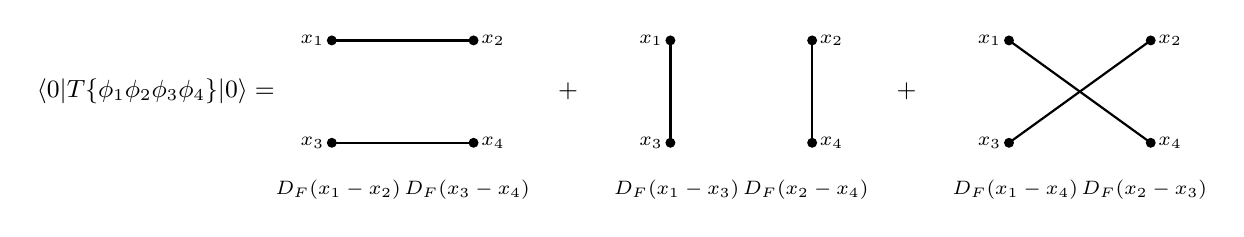
\begin{tikzpicture}[font=\small]
  \foreach \k/\pairs/\lab in {0/{1/2,3/4}/{D_F(x_1-x_2)\,D_F(x_3-x_4)}, 1/{1/3,2/4}/{D_F(x_1-x_3)\,D_F(x_2-x_4)}, 2/{1/4,2/3}/{D_F(x_1-x_4)\,D_F(x_2-x_3)}}{
    \begin{scope}[xshift=\k*4.3cm]
      \coordinate (1) at (0,1.3); \coordinate (2) at (1.8,1.3); \coordinate (3) at (0,0); \coordinate (4) at (1.8,0);
      \foreach \u/\v in \pairs {\draw[fdl] (\u)--(\v);}
      \foreach \n in {1,2,3,4}{\node[fdx] at (\n){};}
      \node[fdlab,left] at (1){$x_1$}; \node[fdlab,right] at (2){$x_2$};
      \node[fdlab,left] at (3){$x_3$}; \node[fdlab,right] at (4){$x_4$};
      \node[font=\scriptsize] at (0.9,-0.6) {$\lab$};
    \end{scope}
  }
  \node at (3.0,0.65) {$+$}; \node at (7.3,0.65) {$+$};
  \node[anchor=east] at (-0.6,0.65) {$\langle0|T\{\phi_1\phi_2\phi_3\phi_4\}|0\rangle=$};
\end{tikzpicture}
